\chapter{Resultados}

En este capítulo se presentan los resultados obtenidos tras la implementación y puesta en marcha del sistema SIVEH en el entorno operativo del verificentro. La evaluación se fundamenta en un análisis mixto que combina métricas cuantitativas de rendimiento y la percepción cualitativa de los usuarios finales recolectada mediante cuestionarios estructurados ver \autoref{anexo:Cuestionarios}.

\section{Optimización de la Eficiencia Operativa}

El impacto más significativo del sistema se observa en la drástica reducción de los tiempos de procesamiento. Al centralizar la información en una arquitectura web, se eliminó la latencia provocada por la consulta de múltiples archivos de Excel y bitácoras físicas.

\begin{figure}[H]
    \centering
    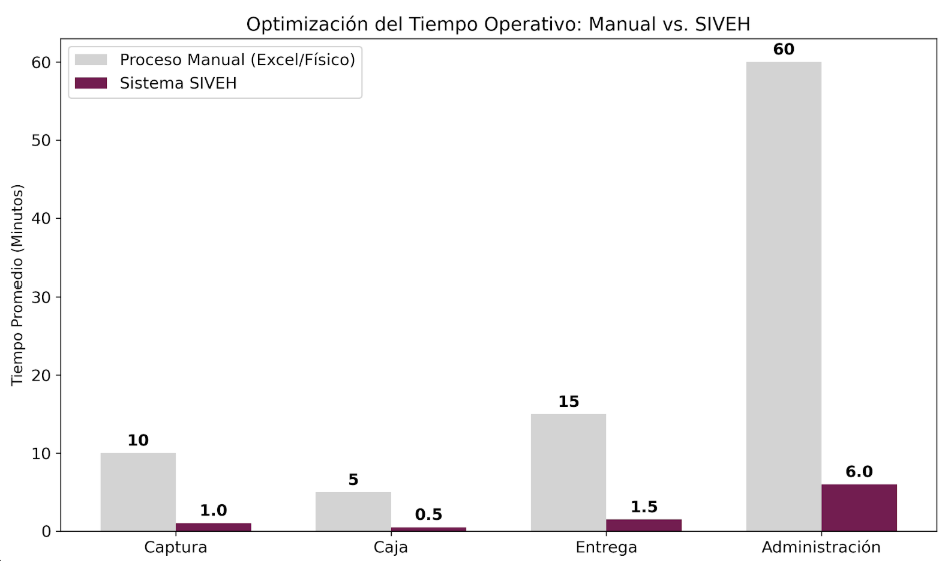
\includegraphics[width=0.7\linewidth]{imagenes/grafico tiempo de operacion.png}
    \caption{Comparativa de tiempos promedio de operación por módulo (en minutos).}
    \label{fig:tiempos_minutos}
\end{figure}

Como se aprecia en la Fig. \ref{fig:tiempos_minutos}, se logró una optimización del 90\% en las tareas críticas. El área administrativa redujo su carga de conciliación de 60 a solo 6 minutos. Los usuarios de caja y captura validaron esta métrica mediante sus testimonios, destacando que \textit{"antes se pasaban horas cuadrando el Excel con lo físico, y ahora con los reportes automáticos todo sale a la primera"}.

\section{Integridad y Confiabilidad de la Información}

La transición de un sistema basado en hojas de cálculo a un motor relacional PostgreSQL permitió blindar la integridad de los datos. Se evaluó la precisión de la información contrastando los registros históricos con los generados por SIVEH.

\begin{figure}[H]
    \centering
    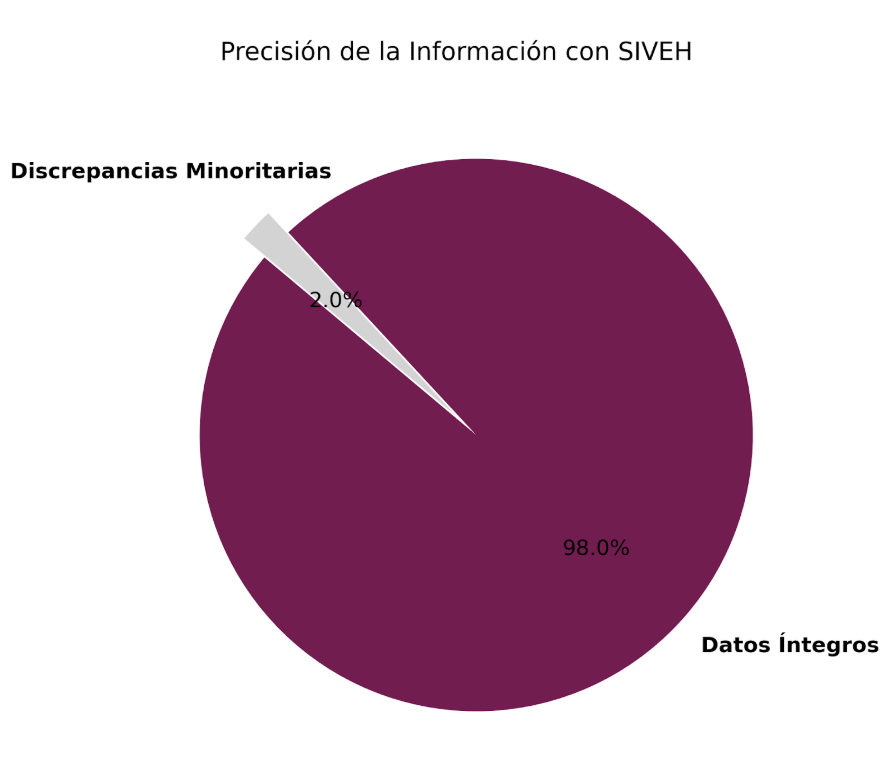
\includegraphics[width=0.7\linewidth]{imagenes/grafico precision.png}
    \caption{Análisis de precisión e integridad de los datos en el ecosistema SIVEH.}
    \label{fig:precision_datos}
\end{figure}

La Fig. \ref{fig:precision_datos} ilustra que el 98\% de la información procesada se mantiene con total integridad. El 2\% de discrepancias detectadas se asocia a la depuración de datos erróneos provenientes del sistema anterior. Esta robustez técnica fue confirmada por el área de entrega de resultados, quienes reportaron una disminución total en los errores de asignación de hologramas, señalando que \textit{"el hecho de que el folio esté amarrado digitalmente al vehículo otorga seguridad al operador y al cliente"}.

\section{Evaluación de la Experiencia de Usuario (UX/UI)}

La aceptación del sistema por parte del personal operativo es un indicador clave del éxito del proyecto. Se evaluaron cuatro pilares fundamentales de la interfaz: facilidad de uso, diseño visual, confianza en los datos y velocidad de respuesta.

\begin{figure}[H]
    \centering
    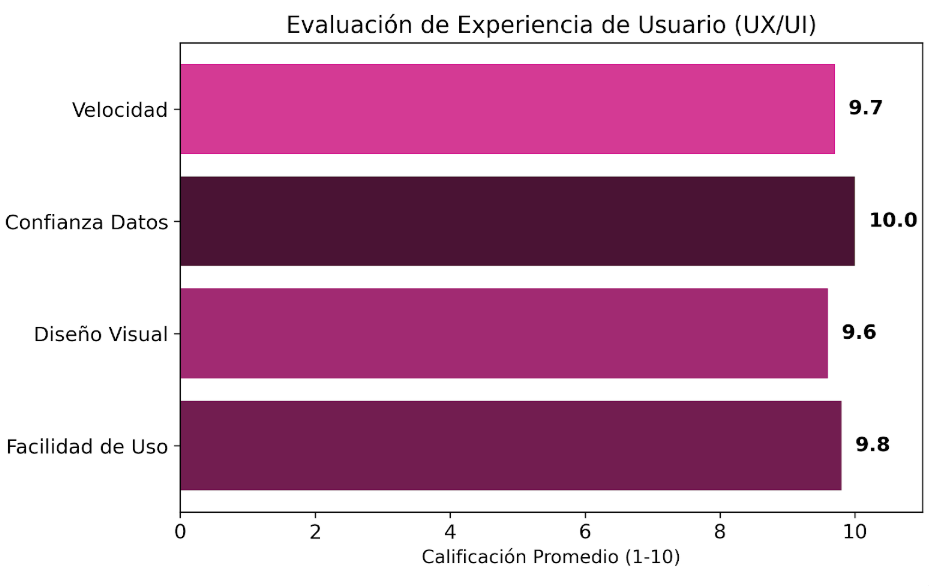
\includegraphics[width=0.7\linewidth]{imagenes/grafico UX.png}
    \caption{Métricas de aceptabilidad y ergonomía de la interfaz de usuario.}
    \label{fig:satisfaccion_ux}
\end{figure}

Los resultados presentados en la Fig. \ref{fig:satisfaccion_ux} muestran una calificación promedio de 9.8/10 en amigabilidad. Los operadores de captura enfatizaron la ergonomía del diseño, mencionando que \textit{"la paleta de colores no cansa la vista durante jornadas prolongadas"}. Asimismo, la disposición lógica de los menús permitió que el sistema fuera intuitivo, eliminando la necesidad de manuales extensos y facilitando la fluidez del trabajo mediante el uso de comandos de teclado.

\section{Impacto en la Gestión Administrativa}

Finalmente, el módulo administrativo demostró ser una herramienta estratégica para la toma de decisiones. La implementación de alertas de inventario en tiempo real y la automatización de los cortes de caja permitieron al administrador reducir a la mitad el tiempo dedicado a la supervisión contable.

Los usuarios de caja destacaron la claridad de los reportes generados: \textit{"Ya no tengo que estar rezando para que no me haya faltado un ticket; el sistema desglosa todo por tipo de pago y el total sale exacto"}. Este nivel de precisión asegura una transparencia total en las finanzas del verificentro y una logística eficiente en la solicitud de nuevos hologramas a la bóveda central.